% !TEX root = Calli.tex
% Kapitelvorlage

\section{Anleitung}
\label{sec:Anleitung}

\subsection{Anwendung mit Kamera-Stream}

Um das Programm mit dem geringsten Aufwand ausführen zu können, wurde mit dem \emph{PyInstaller} aus dem Python-Programm eine .exe - Anwendung erstellt. Diese Version ist auf eine Webcam in 40cm über der Spielfläche bei indirekter Beleuchtung eingestellt, siehe Kapitel \ref{sub:Aufbau}.
\begin{figure}[H]
    \centering
    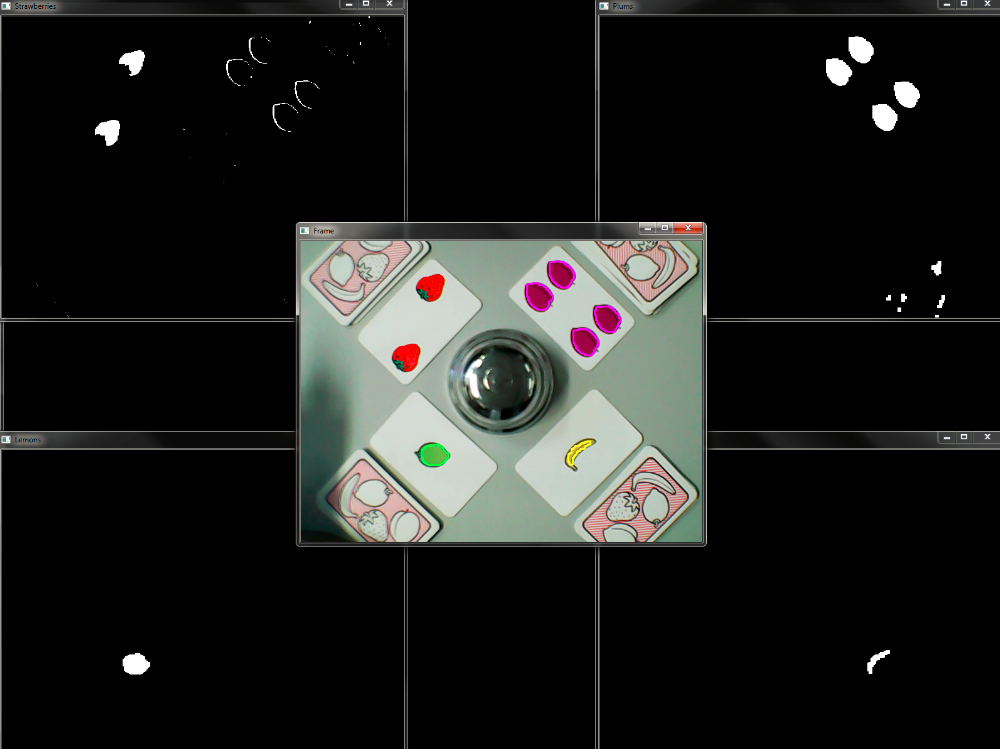
\includegraphics[width=15cm]{Abbildungen/HalliGalli01}
    \caption[Aus]{Bildschirmausgabe der Anwendung mit Kamera-Stream}
    \label{fig:Ausgabe}
\end{figure}
Mit \lstinline{ESC} lässt sich die Anwendung beenden. 

\subsection{Konsolenanwendung für Bilder}
Für Demonstrationszwecke wurde eine Variante als Konsolenanwendung erstellt, um das Programm ohne Kamera mit Beispielbildern zu testen. 
An die Anwendung wird mit dem Kürzel \lstinline{-i} die Bilddatei angehängt.
 
Wahlweise können mit Optionskürzeln zusätzliche Informationen angezeigt werden:
\begin{itemize}
\item \lstinline{-c} zeigt in Weiß die Kontur der umschließenden Rechtecke an. 
\item \lstinline{-o} zeigt die Textausgabe der Werte in der Formsegmentierung an.
\begin{itemize}
\item Verhältnis der detektierten Fläche zur Fläche des umschließenden Rechteckes
\item Verhältnis der Höhe zur Breite des umschließenden Rechteckes
\item Größe der detektierten Fläche
\end{itemize}
\end{itemize}

\begin{singlespace}
\begin{lstlisting}[ ]
cd <programdir>
Calli-Cv-Pictures.exe -i Testbild01.PNG -c -o
\end{lstlisting}
\end{singlespace}
Bei der Ausführung öffen sich vier Fenster mit den Binärbildern zu den einzelnen Früchten und ein Fenster mit dem Originalbild und den darin eingezeichneten Konturen und Texten. Wenn im Bild fünf Früchte einer Sorte detektiert wurden wird dies zusätzlich in der Konsole ausgegeben.

\begin{figure}[H]
    \centering
    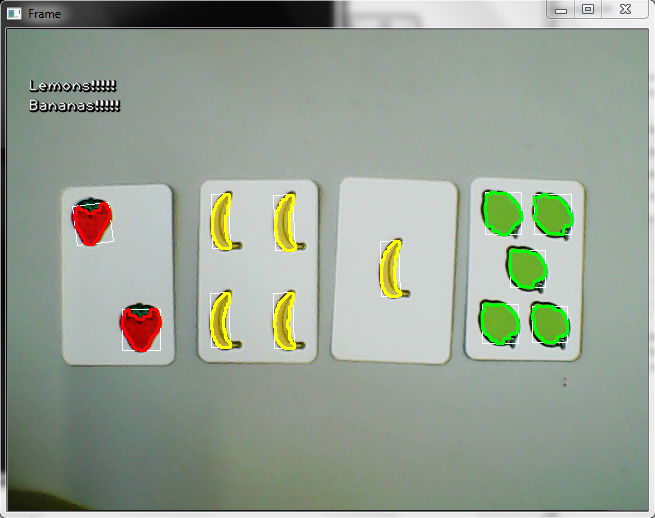
\includegraphics[width=15cm]{Abbildungen/Calli-Konsole}
    \caption[Konsole]{Konsolenanwendung}
    \label{fig:Konsole}
\end{figure}

Nach dem Drücken einer beliebigen Taste schließt sich die Anwendung.